	\documentclass[a4paper, 11pt]{report}

% Packages a utilizar e respetivos parâmetros.
\usepackage[utf8]{inputenc}
\usepackage[portuguese]{babel}
\usepackage{indentfirst}
\usepackage{graphicx}

% Definições das dimensões das páginas
\setlength{\textheight}{24.00cm}
\setlength{\textwidth}{15.50cm}
\setlength{\topmargin}{0.35cm}
\setlength{\headheight}{0cm}
\setlength{\headsep}{0cm}
\setlength{\oddsidemargin}{0.25cm}
\setlength{\evensidemargin}{0.25cm}

%
% Times New Roman font.
%
\usefont{T1}{ptm}{m}{n}
\selectfont

% Title Page
\title{1º Trabalho Prático de Avaliação}
\author{
	\begin{tabular}{ll}
		& Nuno Veloso 42181\\
		& Steven Brito 42798\\
		& Daniela Gomes 42799\\
	\end{tabular}
}


\begin{document}
\maketitle
\cleardoublepage
\begin{center}
	\LARGE
	\textbf{Resumo}
\end{center}
Com o intuito de realizar o 1º trabalho prático da unidade curricular Sistemas Distribuídos pretende-se implementar um sistema distribuído para suportar a troca de mensagens textuais e instantâneas entre pessoas ou grupos num cenário de uma grande área geográfica dividida por regiões.
Ao longo deste trabalho iremos aplicar os conceitos aprendidos nas aulas. Iremos descrever e discutir as vantagens, os problemas e os desafios que se colocam no desenvolvimento deste sistema distribuído.
	
	\chapter{Introdução}
Neste trabalho irá ser desenvolvido um sistema distribuído capaz de trocar mensagens entre utilizadores dentro da mesma região ou entre regiões. Desta forma são precisos vários servidores regionais - um servidor para cada região - e um servidor central. Com esta arquitetura podemos ter cenários em que o servidor central possa falhar e as trocas de mensagens entre regiões não aconteça mas dentro de cada região continue a funcionar. Podemos imaginar outro cenário que seria um servidor regional a falhar. Neste caso só a região desse servidor é que não conseguiria trocar mensagens. Mensagens de outras regiões também não chegariam à região afetada.
	
	\chapter{Descrição do Problema}

O problema consiste em desenvolver um sistema distribuído capaz de trocar mensagens instantâneas, ou seja, sem haver o armazenamento das mesmas, entre utilizadores dentro da mesma região ou entre regiões. É necessário evitar sobrecarga nos servidores. É também necessário garantir que os vários acessos simultâneos aos servidores que mantenham a consistência dos dados. O sistema desenvolvido deve ter em conta tolerância a falhas.
	
	\chapter{Requisitos}
Neste capitulo é descrito os requisitos funcionais do sistema, assim como os não funcionais.
\section{Funcionais}
Os requisitos funcionais deste sistema são os seguintes apresentados:
\begin{itemize}
	\item Evitar sobrecarga no servidor central;
	\item O cliente comunica apenas com o servidor da sua região;
	\item O cliente tem um identificador único;
	\item O cliente conhece todos os servidores regionais;
	\item O cliente regista-se num servidor regional;
	\item O cliente pode enviar mensagens para um único cliente ou para um grupo onde este pertença;
	\item O cliente pode mudar de região;
	\item O cliente pode criar grupos;
	\item O grupo pode ter clientes pertencentes a várias regiões;
	\item Os servidores regionais e centrais devem conhecer a estrutura dos grupos;
	\item Os clientes que não estejam conectados não recebem as mensagens.
\end{itemize}
\section{Não Funcionais}
Os requisitos não funcionais deste sistema são os seguintes apresentados:
\begin{itemize}
	\item 
\end{itemize}
	
	\chapter{Arquitetura}

\section{Interação entre as partes}
Um utilizador apenas interage com o servidor regional onde este está registado. O servidor regional comunica-se com o utilizador e com o servidor central. O servidor central apenas interage com os servidores regionais.

\begin{figure}[h]
	\makebox[\textwidth][c]{
		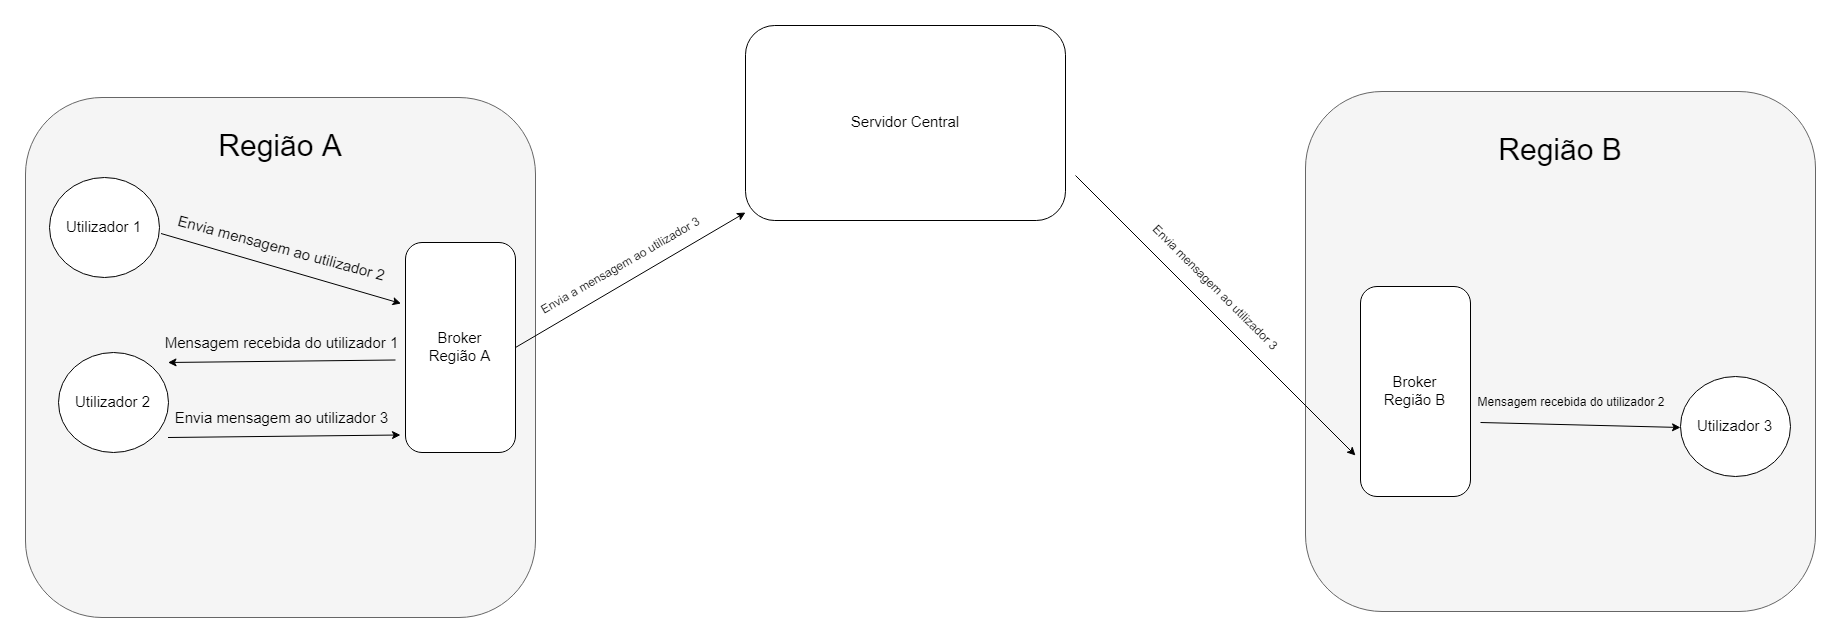
\includegraphics[width=1.3\textwidth]{./figures/diagram}
	}
\end{figure}

O utilizador é cliente do servidor regional. O servidor regional é servidor do utilizador e cliente do servidor central. O servidor central é servidor do servidor regional.

\section{Funcionamento}

Para puder utilizar o sistema, o utilizador deve escolher em qual região pretende-se conectar. Estando este conectado, é possível usufruir das seguintes funcionalidades:
\begin{itemize}
	\item Enviar mensagens para o utilizador;
	\item Criar grupos;
	\item Enviar mensagens para um grupo;
	\item Trocar de regiões;
	\item Sair de uma região.
\end{itemize}

\subsection{Funcionamento entre utilizadores}
Para um utilizador enviar uma mensagem para outro utilizador da mesma região o processo ocorre apenas no servidor dessa região. Caso o utilizador deseje enviar uma mensagem para outro utilizador fora da sua região, o servidor da região irá comunicar-se com o servidor central dizendo para este tratar de enviar a mensagem para um determinado utilizador que o servidor regional não tem conhecimento. O servidor central irá verificar em qual dos servidores regionais está presente o utilizador que tem de receber a mensagem e enviar a mensagem para esse servidor regional. Por sua vez, o servidor regional trata de entregar a mensagem ao utilizador.

\subsection{Funcionamento em grupo}
É possível ao utilizador criar grupos dentro de uma região e adicionar outros utilizadores quer estejam na mesma ou em diferentes regiões. Ao adicionar um utilizador de outra região, a informação desse grupo será replicada para essa região e para todas as outras regiões que contenham informação desse grupo. Apenas o criador do grupo tem permissão para eliminar esse grupo. Aos utilizadores que pertencem a um grupo, estes têm permissão para adicionar outros utilizadores. Os utilizadores que pertencem a um grupo nunca podem sair desse grupo, só sairão quando o criador apagar o grupo.
	
	\chapter{Implementação}

A solução encontra-se dividida em várias aplicações de consola, uma aplicação WinForm e outra em Java. 

\section{KVService} \label{kvservice}

Para ser implementado o servidor de armazenamento, foi necessário definir a interface IKVService, apresentada na figura \ref{ikvservice}.\\ 

\begin{figure}[h]
	\makebox[\textwidth][c]{
		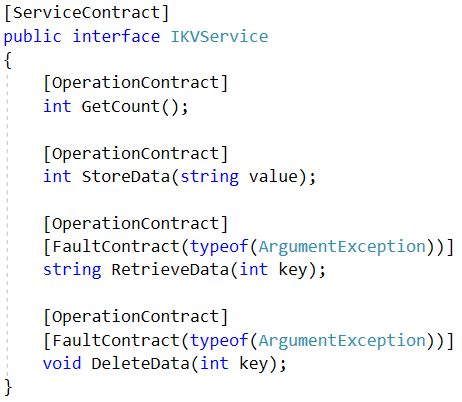
\includegraphics[width=0.7\textwidth]{./figures/ikvservice}
	}
	\caption{Interface IKVService}
	\label{ikvservice}
\end{figure}

O servidor de armazenamento é \textit{stateful} pois tem de guardar os dados de forma persistente. A forma de guardar os dados é em memória.\\
Para a implementação do servidor de armazenamento foi usado o padrão \textit{singleton}. Foi usado este padrão uma vez que é preciso manter estado global.
Os pedidos irão ser atendidos por threads diferentes, pelo que o \textit{ConcurrencyMode} escolhido foi \textit{Multiple}.\\
Assumindo a existência deste serviço na mesma rede com o serviço de \textit{broker}, a comunicação é feita através do protocolo TCP. Foi escolhido este protocolo por ser mais eficiente em relação ao protocolo HTTP e como referido anteriormente, assumindo que ambos os serviços estão na mesma rede. Se mais tarde for requisito estes serviços estarem em redes diferentes, basta mudar o ficheiro de configuração e alterar o \textit{binding} e o \textit{base address} para suportar o protocolo HTTP.

\section{BrokerService} \label{brokerservice}

Para implementar o \textit{broker}, definiu-se a interface IBrokerService, apresentada na figura \ref{ibrokerservice}.

\begin{figure}[h]
	\makebox[\textwidth][c]{
		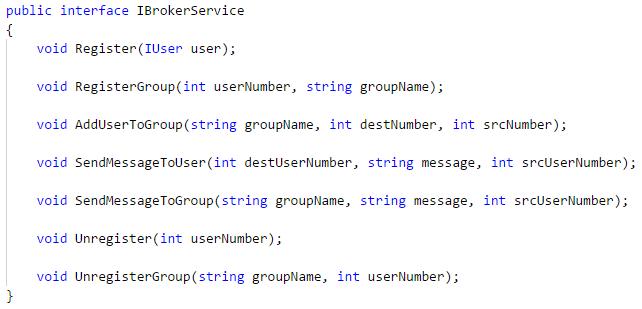
\includegraphics[width=0.7\textwidth]{./figures/ibrokerservice}
	}
	\caption{Interface IBrokerService}
	\label{ibrokerservice}
\end{figure}

Os \textit{brokers} são \textit{stateless} por forma a facilitar o balanceamento de carga. De forma a não ter o objeto em memória foi usado o \textit{InstanceContextMode} \textit{PerCall}.\\
Como o modo é PerCall, ou seja, irá ser criada uma nova instância da classe \textit{BrokerService} a cada chamada, não é necessário garantir controlo de concorrência.\\
Para determinar qual o servidor de armazenamento com maior disponibilidade em termos de volume de dados inseridos, o \textit{broker} pergunta a todos os servidores de armazenamento a carga de cada um. Após ter esta informação, o \textit{broker} ordena os servidores de armazenamento por ordem crescente do volume de dados. Irá escolher os dois primeiros para armazenar o valor nesses servidores. Se algum deles falhar o \textit{broker} tenta guardar no terceiro servidor de armazenamento com menor volume de dados inseridos. Este processo repete-se até conseguir guardar em pelo menos dois servidores de armazenamento. Se conseguir guardar, irá construir um objeto \textit{Key}. Caso contrário irá enviar uma mensagem de exceção a dizer que não foi possível guardar.\\

Para representar a chave de um valor guardado, foi criada a classe \textit{Key} cuja definição se encontra na figura \ref{keydatacontract}

\begin{figure}[h]
	\makebox[\textwidth][c]{
		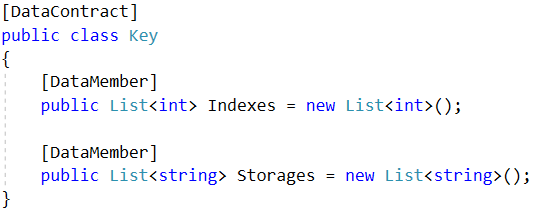
\includegraphics[width=0.7\textwidth]{./figures/key}
	}
	\caption{Classe \textit{Key}}
	\label{keydatacontract}
\end{figure}

Nesta classe é guardada o endereço dos servidores de armazenamento como forma de localização e o índice onde o valor foi guardado dentro do servidor de armazenamento.

Como foi referido na secção \ref{kvservice} é assumido a existência do \textit{broker} na mesma rede que o serviço descrito nessa secção. O \textit{broker} comunica diretamente com o servidor de armazenamento, logo o \textit{binding} usado deve ser o mesmo.
Para que o serviço exposto pelo \textit{broker} seja acessível fora da própria rede, foi usado o protocolo HTTP. O \textit{binding} usado foi o \textit{BasicHttpBinding} porque não é necessário manter sessão ou permitir \textit{callbacks}.

\section{Controlo de Concorrência} \label{concorrencia}

Como o servidor de armazenamento segue o padrão \textit{singleton} irá atender os diferentes pedidos em diferentes \textit{threads}. Como as \textit{threads} irão aceder à mesma instância, é necessário garantir controlo de concorrência. Para garantir o acesso concorrente ao estado dessas instâncias, foi usado a biblioteca \textit{Concurrent} do .NET.\\

\section{Ficheiros de Configuração} \label{configuracao}

De forma a não comprometer o código com os URLs, protocolos, implementações e \textit{bindings}, foi usado ficheiros de configuração.
	
	\chapter{Tolerância a Falhas}

Com esta arquitetura existem cenários em que o servidor central possa falhar e as trocas de mensagens entre regiões não aconteça, mas que dentro de cada região continue a funcionar. Mesmo se o servidor central voltar a conectar-se, não irá realizar uma nova conexão aos servidores regionais já existentes, estes funcionarão independentemente da nova instância do servidor central. O problema causado por isso é não permitir interação entre regiões. Estes servidores regionais ficarão com uma instância de um servidor central que já não está conectado. Esta solução permite a troca de mensagens entre utilizadores dentro da mesma região. Uma outra solução passaria por desconectar todos os servidores regionais e instanciá-los novamente após o servidor central ser instanciado. Esta solução implicaria perder todos os dados de utilizadores e de grupos já registados nos servidores regionais.\\

Um outro cenário seria um servidor regional a falhar. Neste caso só a região desse servidor é que não conseguiria trocar mensagens. Mensagens de outras regiões também não chegariam à região afetada. Caso o servidor central envie mensagens para este servidor regional, tal não é possível, pois este servidor foi desconectado. Esta solução tem um inconveniente. O servidor central tem guardado informação de servidores regionais que podem já não estar conectados. O servidor central não tem maneira de identificar se o servidor regional foi desconectado ou se é um problema de comunicação.
Uma solução alternativa passaria por contar o número de chamadas consecutivas que o servidor central faz ao servidor regional e este não responde com sucesso. Teria de ser atribuído um número máximo de chamadas consecutivas falhadas, e eliminar a informação deste servidor regional no servidor central, após o número de chamadas ultrapassar o limite. O problema com esta solução é que o servidor regional poderia estar novamente disponível após o limite de tentativas, e assim o servidor central iria apagar informação de um servidor regional ativo.\\

Semelhante aos servidores regionais, se um cliente desconectar-se sem informar o servidor regional de que irá desconectar-se, os dados ficam guardados tanto neste como no servidor central. O problema para determinar se o utilizador está ativo ou apenas com problemas de comunicação é o mesmo descrito no parágrafo anterior, portanto a solução é idêntica à utilizada nos servidores regionais.
	
	\chapter{Manual de utilização} \label{manual}

Para usar o sistema desenvolvido, terá de executar os seguintes passos dentro da pasta Install:

\begin{enumerate}
	\item Lançar o executável \textit{CentralManagerServer.exe} que consta dentro da pasta Central Manager;
	\item Dentro da pasta Brokers, existem duas pastas. Em cada uma delas, deverá lançar o executável \textit{BrokerServer.exe};
	\item Para executar um ou mais clientes, deverá lançar o executável \textit{UserFormImpl.exe} presente na pasta User, consoante o número de utilizadores desejado.
\end{enumerate}

\section{Utilização do Cliente}

\begin{figure}[h]
	\makebox[\textwidth][c]{
		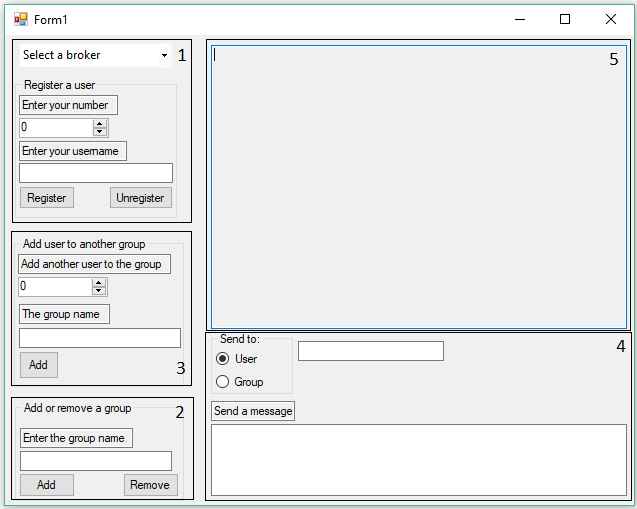
\includegraphics[width=0.9\textwidth]{./figures/form}
	}
	\caption{User Form}
	\label{form}
\end{figure}

Na figura \ref{form} é apresentada a interface gráfica do utilizador.
Relativamente a esta figura, existem retângulos numerados. Cada retângulo é explicado de seguida.\\

No retângulo 1, pode selecionar o \textit{broker} à qual o utilizador pretende-se registar. Para tal, necessita de indicar o seu número e o seu nome. Para se registar, deve preencher o formulário e carregar no botão \textit{Register}. Para fazer \textit{Unregister}, deve carregar no botão \textit{Unregister}.\\

No retângulo 2, existe a possibilidade de criar ou remover grupos. Para criar ou remover um grupo, basta indicar o seu nome e carregar no botão \textit{Add} ou \textit{Remove} para adicionar ou remover um grupo, respetivamente.\\

No retângulo 3, pode adicionar um utilizador a um dado grupo à qual pertence. Para realizar esta operação, deverá indicar o número do utilizador que pretende adicionar e o nome do grupo ao qual irá adicionar. Havendo preenchido o formulário, deverá carregar no botão \textit{Add}.\\

O retângulo 4, permite enviar mensagens para um utilizador ou para um grupo. Para enviar uma mensagem para um utilizador, deverá selecionar o \textit{radio button User} e indicar o número do utilizador à qual pretende enviar a mensagem. A caixa de texto \textit{Send a message} permite escrever a mensagem que pretende enviar. Para enviar, basta pressionar o botão do teclado \textit{Enter}. Se pretender enviar a mensagem para um grupo, o procedimento repete-se, diferindo apenas na escolha do \textit{radio button}, que deverá ser \textit{Group}.\\

O retângulo 5 é onde se apresenta as mensagens enviadas e recebidas, quer por utilizadores, quer por grupos. As mensagens vêm identificadas pelo nome do utilizador caso exista. Caso contrário, são identificadas pelo número do utilizador. 
	
\end{document}          
